\chapter{Strateegiline analüüs}
Selles peatükis vaadeldakse tervet infosüsteemi, leitakse selle allsüsteemid ning esitatakse ühele põhiobjektile vastava funktsionaalse allsüsteemi/registri paari eskiismudelid.

\section{Terviksüsteemi üldvaade}
Järgnevalt esitatakse ülevaade autorendi ettevõtte infosüsteemi toimimisest.

\subsection{Organisatsiooni eesmärgid}
\begin{itemize}
	\item Teenida omanikele kasumit
	\item Pakkuda head ja kiiret teenindust, mis jätaks klientidele hea mulje ning suurendaks võimalust, et nad saavad püsiklientideks ja soovitavad pakutavaid teenuseid ka oma tuttavatele
	\item Olla kõigile osapooltele usaldusväärne lepingupartner
	\item Pakkuda klientidele võimalikult laia valikut erinevat liiki sõidukeid
	\item Hoida ettevõtte autopark tehniliselt heas korras ja kaasaegne
	\item Pakkuda ettevõtte töötajatele positiivset ja tunnustust pakkuvat sisekliimat
	\item Pakkuda teenust kliendile just seal, kus ta seda kõige enam vajab
\end{itemize}

\subsection{Infosüsteemi eesmärgid}
\begin{itemize}
	\item Saada ülevaade organisatsiooniga seotud isikutest
	\item Saada ülevaade organisatsiooni töötajatest
	\item Saada ülevaade organisatsiooni klientidest
	\item Saada ülevaade organisatsiooni sõlmitud lepingutest
	\item Võimaldada klassifikaatorite abil andmete liigitamist ja seostamist seostamiseks väljaspool organisatsiooni vastutusala oleva informatsiooniga
	\item Saada ülevaade autodest, millega tehingute (transaktsioonide) tegemine on üks organisatsiooni põhieesmärk
	\item Saada ülevaade organisatsiooni käsutuses olevatest varadest
	\item Võimaldada organisatsioonil luua vara tarnetellimusi
	\item Saada ülevaade organisatsiooni töötajate töögraafikust
	\item Saada ülevaade vabadest autodest
	\item Saada ülevaade kasutusel olevatest autodest
	\item Saada ülevaade organisatsiooniga seotud lepingupartneritest
	\item Võimaldada hallata hinnakirja
	\item Saada ülevaade autode rikete ajaloo kohta
	\item Võimaldada autosid rutiinselt hooldusse saata
	\item Saada ülevaade autode kindlustuslepingutest
	\item Saada ülevaade autode tehnilise ülevaatusese seisundist
	\item Võimaldada klientidel autosid rentida
	\item Võimaldada rentimist tühistada
	\item Võimaldada jälgida autode tagastamisi
	\item Võimaldada pakkuda kliendile sobivat lisavarustust
	\item Saada ülevaade kliendi minevikust
	\item Võimaldada esitada kahjunõudeid
	\item Võimaldada esitada arveid
	\item Võimaldada kliendil jätta tagasiside oma rendikogemuse kohta
	\item Võimaldada klientidele pakkuda soodustusi
	\item Saada ülevaade organisatsioonile tehtud ettekirjutustest
\end{itemize}

\subsection{Lausendid}
\begin{itemize}
	\item Isikul on hetkeseisund
	\item Isiku seisundi liik on klassifikaator
	\item Töötaja on isik
	\item Töötajal on hetkeseisund
	\item Töötaja seisundi liik on klassifikaator
	\item Töötaja töötab ametis
	\item Amet on klassifikaator
	\item Juhataja on töötaja
	\item Autode haldur on töötaja
	\item Klient on isik
	\item Kliendil on hetkeseisund
	\item Uudistaja on süsteemi tuvastamata kasutaja
	\item Kliendi seisundi liik on klassifikaator
	\item Juhataja on organisatsiooni omanik
	\item Autode haldur haldab autosid
	\item Klassifikaatorite haldur haldab klassifikaatoreid
	\item Klienditeenindaja on töötaja
	\item Autojuht on töötaja
	\item Raamatupidaja on lepingupartner
	\item Klient sõlmib lepingu
	\item Lepingul on hetkeseisund
	\item Lepingu seisundi liik on klassifikaator
	\item Töötaja registreerib auto
	\item Autot iseloomustab null või rohkem kategooriat
	\item Auto kategooria on klassifikaator
	\item Autol on hetkeseisund
	\item Auto seisundi liik on klassifikaator
	\item Organisatsioonil on hetke seisund
	\item Organisatsiooni seisundi liik on klassifikaator
	\item Organisatsioon võib olla klient
	\item Töötajal on töögraafik
	\item Töögraafikul on hetkeseisund
	\item Töögraafiku hetkeseisund on klassifikaator
	\item Auto on hinnastatud hinnakirja alusel
	\item Hinnakirjal on hetkeseisund
	\item Hinnakirja seisundi liik on klassifikaator
	\item Lisavarustusel on hetkeseisund
	\item Lisavarustuse seisundi liik on klassifikaator
	\item Rentimisel on hetkeseisund
	\item Rentimise seisundi liik on klassifikaator
	\item Soodustusel on hetkeseisund
	\item Soodustuse seisundi liik on klassifikaator
	\item Kindlustusleping on iga auto kohta eraldi
	\item Kindlustuslepingul on hetkeseisund
	\item Kindlustuslepingu seisundi liik on klassifikaator
	\item Ülevaatus on iga auto kohta eraldi
	\item Ülevaatusel on hetkeseisund
	\item Ülevaatuse seisundi liik on klassifikaator
	\item Arvel on hetkeseisund
	\item Arve seisundi liik on klassifikaator
	\item Kahjunõudel on hetkeseisund
	\item Kahjunõude seisundi liik on klassifikaator
	\item Inventuuril on hetkeseisund
	\item Inventuuri seisundi liik on klassifikaator
	\item Rikkel on hetkeseisund
	\item Rikke seisundi liik on klassifikaator
	\item Hooldusel on hetkeseisund
	\item Hoolduse seisundi liik on klassifikaator
	\item Vara tarnetellimusel on hetkeseisund
	\item Vara tarnetellimuse seisundi liik on klassifikaator
	\item Lepingupartner on teine organisatsioon
	\item Lepingupartneril on hetkeseisund
	\item Lepingupartneri seisundi liik on klassifikaator
	\item Lepingupartner sõlmib lepingu
	\item Tagasisidel on hetkeseisund
	\item Tagasiside seisundi liik on klassifikaator
	\item Organisatsioonile tehakse ettekirjutus 
	\item Ettekirjutusel on hetkeseisund
	\item Ettekirjutuse seisundi liik on klassifikaator
	\item Ettekirjutuse koostab andmekaitse inspektsioon
\end{itemize}

\subsection{Põhiobjektid}
\begin{itemize}
	\item Isik
	\item Organisatsioon
	\item Töötaja
	\item Klient
	\item Klassifikaator
	\item Töögraafik
	\item Leping
	\item Auto
	\item Hinnakiri
	\item Lisavarustus
	\item Rentimine
	\item Soodustus
	\item Kindlustusleping
	\item Ülevaatus
	\item Arve
	\item Kahjunõue
	\item Inventuur
	\item Rike
	\item Hooldus
	\item Vara tarnetellimus
	\item Lepingupartner
	\item Tagasiside
	\item Ettekirjutus
\end{itemize}

\subsection{Põhiprotsessid}
\begin{itemize}
	\item Isiku registreerimine
	\item Isiku surnuks märkimine
	\item Töötaja tööle võtmine
	\item Töötaja ametikoha muutmine
	\item Töötaja ajutiselt töölt vabastamine
	\item Töötaja puhkusele siirdumine
	\item Klassifikaatori väärtuse lisamine
	\item Klassifikaatori väärtuse muutmine
	\item Lepingu sõlmimine
	\item Lepingu peatamine
	\item Lepingu ühepoolne katkestamine
	\item Lepingu pikendamine
	\item Auto registreerimine
	\item Auto unustamine
	\item Auto aktiveerimine
	\item Auto ajutiselt kasutusest eemaldamine (mitteaktiivseks muutmine)
	\item Auto lõplikult kasutusest eemaldamine (lõpetamine)
	\item Töögraafiku määramine töötajale
	\item Hinnakirjas muudatuste tegemine
	\item Lisavarustuse pakkumine 
	\item Sõiduki rentimine kliendile
	\item Soodustuse pakkumine kliendile
	\item Auto kindlustuslepingu olemasolu kontrollimine
	\item Auto ülevaatuse olemasolu kontrollimine
	\item Arve esitamine rentimise eest
	\item Arve makseseisundi kontrollimine
	\item Kahjunõude esitamine
	\item Inventuuri tegemine
	\item Rikke talletamine auto ajalukku
	\item Auto hooldusele saatmine
	\item Auto tehnilise ülevaatuse seisundi uuendamine
	\item Auto tehnilisse ülevaatusse saatmine
	\item Uue lepingupartneriga lepingu sõlmimine
	\item Tagasiside saamine
	\item Tagasiside põhjal otsuste langetamine
	\item Ettekirjutuse saamine
\end{itemize}

\subsection{Põhilised sündmused}
\begin{itemize}
	\item Organisatsiooni vaatevälja satub uus isik, kellega organisatsioon soovib  astuda mingil viisil lepingulistesse suhetesse
	\item Isik sureb
	\item Organisatsiooni tuleb tööle uus töötaja
	\item Töötaja liigub karjääriredelil
	\item Töötajat hakatakse kahtlustama organisatsiooni huve kahjustavas teos
	\item Töötaja võtab välja kasutamata puhkuse
	\item Tekib vajadus uue klassifikaatori väärtuse lisamiseks (nt tänu sellele, et täienes rahvusvaheline standard või tänu sellele, et ettevõtte äriprotsesse otsustati muuta)
	\item Selgus, et klassifikaatori väärtuse registreerimisel oli tehtud viga
	\item Huvitatud osapool (isik või organisatsioon) soovib astuda organisatsiooniga vastastikku kasulikesse lepingulistesse suhetesse
	\item Vähemalt üks lepingu osapooltest teatab, et ta pole ajutiselt võimeline lepingus toodud tingimusi täitma
	\item Vähemalt üks lepingu osapooltest teatab, et ta pole püsivalt võimeline lepingus toodud tingimusi täitma
	\item Lepingu osapooled on oma lepingulise suhtega rahul ja soovivad selle pikendamist
	\item Organisatsiooni jõuab teave uue auto kohta
	\item Selgus, et organisatsiooni jõudnud teave auto kohta on enneaegne ning sellisel kujul autot ei ole vaja registreerida
	\item On vaja muuta võimalikuks auto kasutamine tehingutes
	\item Auto kasutamine tehingutes on vaja ajutiselt peatada, kuna seoses autoga on ilmnenud ajutise iseloomuga probleemid
	\item Auto kasutamine tehingutes on vaja lõpetada, kuna seoses autoga on ilmnenud püsiva iseloomuga probleemid või kuna auto on oma aja lihtsalt ära elanud
	\item Töötajatele on tarvis luua järgneva kuu töögraafik
	\item Turul on konkurentsitingimused muutunud ja vaja hinnakirja kaasajastada
	\item Klient soovib autoga kaasa saada lisavarustust
	\item Auto antakse üle kliendi käsutusse 
	\item Kliendile pakutakse auto rentimist soodustingimuste alusel
	\item Veendumaks, et sõidukitel on kehtiv liikluskindlustus tehakse regulaarset kontrolli kindlustuse seisundi üle
	\item Veendumaks, et sõidukitel on kehtiv ülevaatus tehakse regulaarset kontrolli ülevaatuse seisundi üle
	\item Rendilepingu sõlmimise järel kliendiga esitatakse kliendile arve müüdavate teenuste eest
	\item Enne kliendile auto üle andmist on vaja veenduda, et klient on rentimise eest arve tasunud
	\item Klient on rikkunud ettevõttele kuuluvat vara ning peab hüvitama tekitatud kahjud
	\item Organisatsiooni varade üle arve pidamiseks on tarvis regulaarselt inventuuri teostada
	\item Autoga juhtus õnnetus ning rike on vaja talletada auto ajalukku
	\item Hoidmaks ettevõtte pakutavate teenuste kvaliteeti kõrgel tuleb rutiinselt autosid hooldada
	\item Auto on läbinud tehnilise ülevaatuse ning tohib taas teedel sõita
	\item Auto tehniline ülevaatus on aegumas ning sõidukiga tehingute jätkamiseks tuleb autol sooritada tehniline ülevaatus
	\item Ettevõtte on tellinud uue sõiduki, millega tehinguid teha, ning andmed sõiduki ostu kohta tuleb talletada süsteemi
	\item Ettevõte on alustanud koostööd uue organisatsiooniga ning andmed partnerluse kohta tuleb talletada süsteemi
	\item Rentnik annab kasutatud teenuste kohta tagasisidet ning seda tuleb süsteemis hoida edasiselt paremate otsuste langetamiseks
	\item Süsteemi on talletatud tagasiside ning selle põhjal tehakse otsus tulevikus parema teenuse osutamiseks
	\item Andmekaitse inspektsioon teeb ettevõttele ettekirjutuse ning sellele on vaja reageerida
\end{itemize}

\subsection{Tegutsejad}
\begin{itemize}
	\item Juhataja (ka omanik)
	\item Autode haldur
	\item Klassifikaatorite haldur
	\item Klient
	\item Uudistaja
	\item Autojuht
	\item Klienditeenindaja
	\item Raamatupidaja
\end{itemize}

\subsection{Asukohad}
\begin{itemize}
	\item Kliendid (on süsteemis registreeritud) ja uudistajad (veebikülalised; tuvastamata kasutajad) kasutavad veebirakendust, mille poole pöördumiseks on vaja arvutit, veebilehitsejat ja veebiühendust.
	\item Töötajad töötavad neile spetsiaalselt ettenähtud ruumides. Igale töötajale on ettenähtud oma arvuti. 
\end{itemize}

\subsection{Terviksüsteemi tükeldus allsüsteemideks}
Järgnevalt esitatakse infosüsteemi jaotus kolme erinevat liiki allsüsteemideks.
\\
\par
Organisatsiooni sisesed pädevusalad.
\begin{itemize}
	\item Juhataja
	\item Autode haldur
	\item Klassifikaatorite haldur
	\item Autojuht
	\item Klienditeenindaja
\end{itemize}

Organisatsiooni välised pädevusalad.
\begin{itemize}
	\item Juhataja
	\item Uudistaja
	\item Raamatupidaja
\end{itemize}

\textbf{Tabel 2} esitab sisulised funktsionaalsed allsüsteemid ja nende teenidatavad registrid (seotud organisatsiooni põhitegevusega). %TODO: Improve formatting

\begin{table}[H] % [H] prevents table from floating around
	\caption{\textbf{Tabel 2 Sisulised allsüsteemid.}}
	\begin{tabular}{|l|l|}
		\hline
		\rowcolor[HTML]{C0C0C0} 
		\multicolumn{1}{|c|}{\cellcolor[HTML]{C0C0C0}\textbf{Funktsionaalne allsüsteem}} & \multicolumn{1}{c|}{\cellcolor[HTML]{C0C0C0}\textbf{\begin{tabular}[c]{@{}c@{}}Register, mida see funktsionaalne \\ allsüsteem teenindab\end{tabular}}} \\ \hline
		Klientide funktsionaalne allsüsteem                                              & Klientide register                                                                                                                                      \\ \hline
		Autode funktsionaalne allsüsteem                                                 & Autode register                                                                                                                                         \\ \hline
		Hinnakirja funktsionaalne allsüsteem                                             & Hinnakirja register                                                                                                                                     \\ \hline
		Lisavarustuse funktsionaalne allsüsteem                                          & Lisavarustuse register                                                                                                                                  \\ \hline
		Rentimise funktsionaalne allsüsteem                                              & Rentimiste register                                                                                                                                     \\ \hline
		Soodustuste funktsionaalne allsüsteem                                            & Soodustuste register                                                                                                                                    \\ \hline
		Kahjunõuete funktsionaalne allsüsteem                                            & Kahjunõuete register                                                                                                                                    \\ \hline
		Rikete funktsionaalne allsüsteem                                                 & Rikete register                                                                                                                                         \\ \hline
		Tagasiside funktsionaalne allsüsteem                                             & Tagasiside register                                                                                                                                     \\ \hline
	\end{tabular}
\end{table}

\textbf{Tabel 3} esitab administratiivsed funktsionaalsed allsüsteemid ja nende teenidatavad registrid (võivad olla kasutusel paljudes erinevate eesmärkide ja tegevusaladega organisatsioonides).

\begin{table}[H]
	\caption{\textbf{Tabel 3 Administratiivsed allsüsteemid.}}
	\begin{tabular}{|l|l|}
		\hline
		\rowcolor[HTML]{C0C0C0} 
		\multicolumn{1}{|c|}{\cellcolor[HTML]{C0C0C0}\textbf{Funktsionaalne allsüsteem}} & \multicolumn{1}{c|}{\cellcolor[HTML]{C0C0C0}\textbf{\begin{tabular}[c]{@{}c@{}}Register, mida see funktsionaalne \\ allsüsteem teenindab\end{tabular}}} \\ \hline
		Isikute funktsionaalne allsüsteem                                                & Isikute register                                                                                                                                        \\ \hline
		Töötajate funktsionaalne allsüsteem                                              & Töötajate register                                                                                                                                      \\ \hline
		Klassifikaatorite funktsionaalne allsüsteem                                      & Klassifikaatorite register                                                                                                                              \\ \hline
		Lepingute funktsionaalne allsüsteem                                              & Lepingute register                                                                                                                                      \\ \hline
		Organisatsioonide funktsionaalne allsüsteem                                      & Organisatsioonide register                                                                                                                              \\ \hline
		Töögraafiku funktsionaalne allsüsteem                                            & Töögraafiku register                                                                                                                                    \\ \hline
		Kindlustuste funktsionaalne allsüsteem                                           & Kindlustuste register                                                                                                                                   \\ \hline
		Ülevaatuste funktsionaalne allsüsteem                                            & Ülevaatuste register                                                                                                                                    \\ \hline
		Inventuuri funktsionaalne allsüsteem                                             & Inventuuri register                                                                                                                                     \\ \hline
		Hoolduse funktsionaalne allsüsteem                                               & Hoolduste register                                                                                                                                      \\ \hline
		Vara tarnetellimuste funktsionaalne allsüsteem                                   & Vara tarnetellimuste register                                                                                                                           \\ \hline
		Lepingupartnerite funktsionaalne allsüsteem                                      & Lepingupartnerite register                                                                                                                              \\ \hline
		Arvete funktsionaalne allsüsteem                                                 & Arvete register                                                                                                                                         \\ \hline
		Ettekirjutuste funktsionaalne allsüsteem                                         & Ettekirjutuste register                                                                                                                                 \\ \hline
	\end{tabular}
\end{table}

\newpage
\section{Autode funktsionaalse allsüsteemi eskiismudelid}
Järgnevalt esitatakse eskiismudelid, mida detailanalüüsi käigus täpsustatakse ja täiendatakse.

\subsection{Eesmärgid}
\begin{itemize}
	\item Muuta võimalikuks auto kasutamine erinevates tehingutes (transaktsioonides), mille läbiviimist infosüsteem toetab
	\item Võimaldada auto elektrooniliselt registreerida
	\item Võimaldada määrata auto hetkeseisundit vastavalt elutsüklile
	\item Võimaldada muuta süsteemile teadaolevaid andmeid auto kohta
	\item Võimalik auto andmed kustutada e infosüsteemi mõttes unustada, kuid teha seda ainult siis, kui auto pole veel kordagi aktiivsesse kasutusse läinud
	\item Võimaldada vastata fikseeritud päringutele auto kohta
	\item Võimaldada vaadata määratud elutsüklis olevate autode andmeid
	\item Võimaldada auto kategoriseerimist klassifikaatorite abiga
	\item Võimaldada saada ülevaade kogu autopargi kohta
\end{itemize}

\subsection{Allsüsteemi kasutavad pädevusalad}
\begin{itemize}
	\item Juhataja
	\item Autode Haldur
	\item Uudistaja
	\item Klient
	\item Klassifikaatorite haldur
	\item Autojuht
	\item Klienditeenindaja
\end{itemize}

\subsection{Allsüsteemi poolt vajatavad registrid}
Allsüsteem teenindab autode registrit.
\\
\par
Allsüsteem loeb.
\begin{itemize}
	\item Isikute register
	\item Töötajate register
	\item Klassifikaatorite register
	\item Klientide register
\end{itemize}

\subsection{Allsüsteemi ühe põhiprotsessi tegevusdiag}

\textbf{Joonis 1} esitab auto lõpetamise protsessi kirjelduse tegevusdiagrammina. 
\begin{figure}[H]
	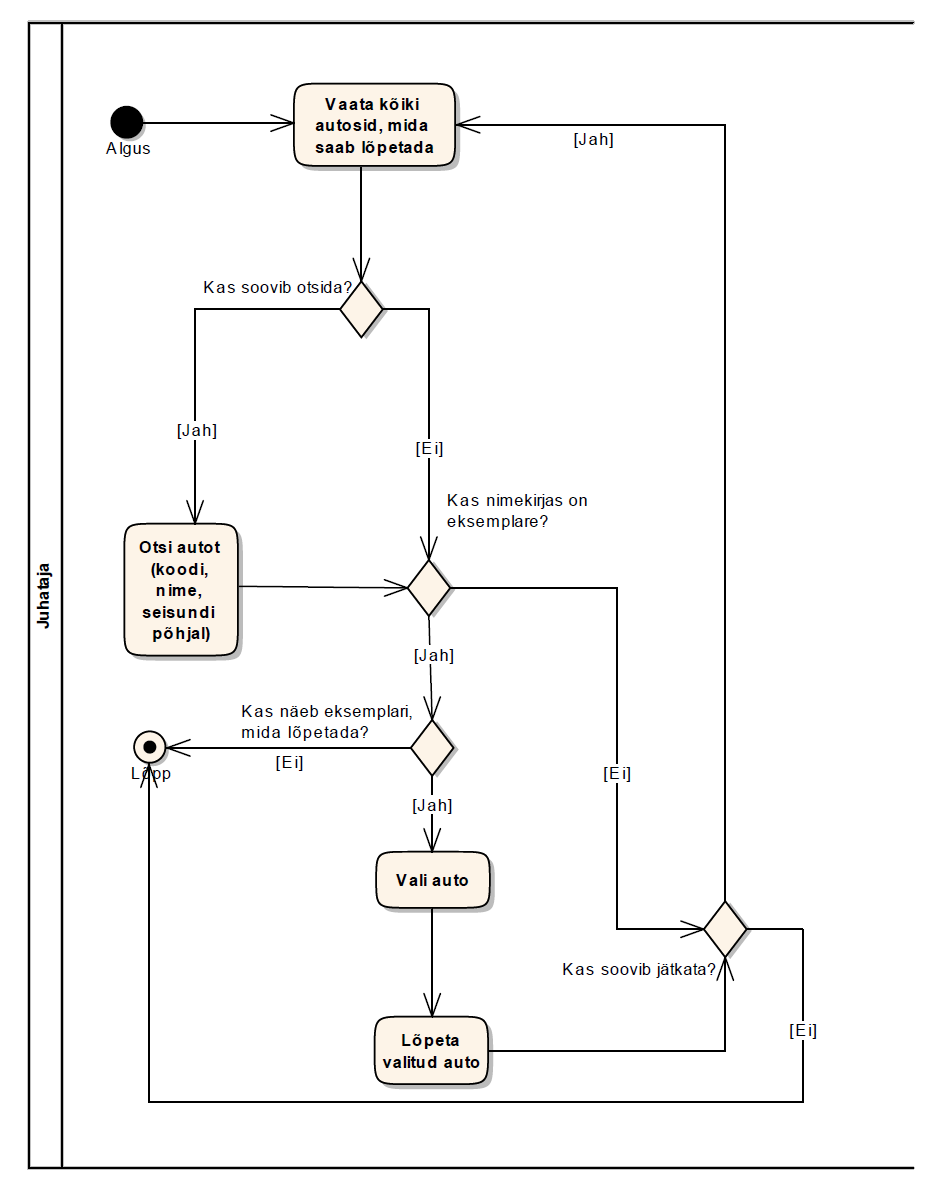
\includegraphics[scale=0.6]{joonis1}
	\caption{\textbf{Joonis 1 Auto lõpetamise tegevusdiagramm.}}
\end{figure}

\subsection{Allsüsteemi kasutusjuhtude eskiismudel}
\textbf{Joonis 2} esitatud kasutusjuhtude diagrammil on värvidel järgmine tähendus.

\begin{itemize}
	\item \colorbox{yellow}{Kollasega} on tähistatud põhikasutusjuhud.
	\item \textbf{\textcolor{orange}{Oranžiga}} on tähistatud abistavad kasutusjuhud (sisuliselt kasutusjuhu fragmendid), mis on kirja pandud selleks, et mitte kirjeldada mitmekordselt erinevates kasutusjuhtudes esinevat ühesugust funktsionaalsust.
	\item \textbf{\colorbox{light-gray}{Halliga}} on tähistatudkasutusjuhud, mis esitavad läbivaid huvisid ning on seotud rohkem kui ühe funktsionaalse allsüsteemiga.
\end{itemize}

\begin{figure}[H]
	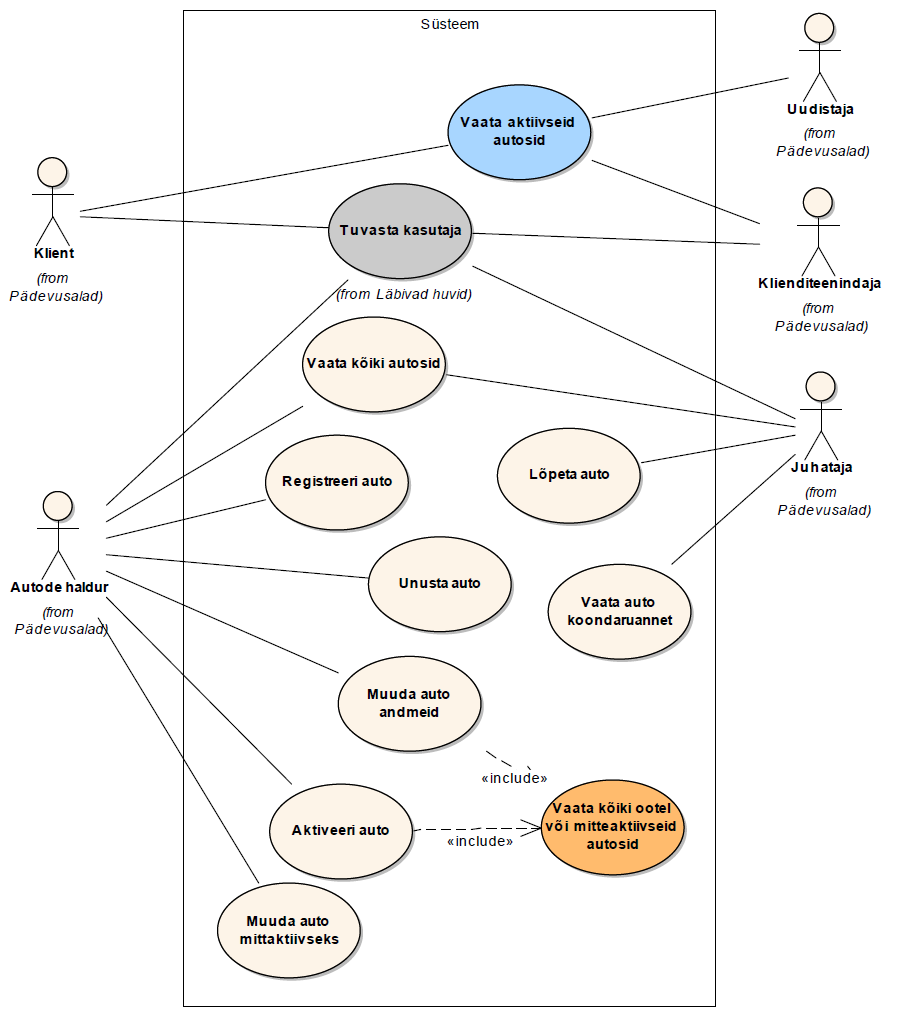
\includegraphics[scale=0.6]{joonis2}
	\caption{\textbf{Joonis 2 Auto funktsionaalse allsüsteemi kasutusjuhtude diagramm.}}
\end{figure}

\begin{flushleft}
\underline{\textbf{Kasutusjuht}: Tuvasta kasutaja} \\
\textbf{Tegutsejad}: Autode haldur, Klienditeenindaja, Juhataja, Klient – (edaspidi Subjekt) \\
\textbf{Kirjeldus}: Subjekt identifitseerib ennast. Selleks sisestab ta kasutajanime, parooli ja oma rolli süsteemis. Süsteem autendib subjekti, st kontrollib subjekti väidetavat identiteeti. Süsteemi sisenemiseks peab subjekt olema ka sobivas seisundis. Kui subjekt on autenditud (isik on tuvastatud ja identiteet kontrollitud), siis lubatakse subjekt süsteemi siseneda, vastasel juhul mitte. Lisaks autoriseeritakse subjekt, andes talle juurdepääsu infosüsteemi objektidele.
\end{flushleft}

\begin{flushleft}
\underline{\textbf{Kasutusjuht}: Registreeri auto} \\
\textbf{Tegutsejad}: Autode haldur \\
\textbf{Kirjeldus}: Autode haldur registreerib uue auto. 
\end{flushleft}

\begin{flushleft}
	\underline{\textbf{Kasutusjuht}: Unusta auto} \\
	\textbf{Tegutsejad}: Autode haldur \\
	\textbf{Kirjeldus}: Autode haldur vaatab ootel autode nimekirja, valib sealt auto ja kustutab selle andmebaasist. Subjekt saab nimekirja sorteerida ja filtreerida. 
\end{flushleft}

\begin{flushleft}
	\underline{\textbf{Kasutusjuht}: Muuda auto andmeid} \\
	\textbf{Tegutsejad}: Autode haldur \\
	\textbf{Kirjeldus}: Autode haldur vaatab ootel  või mitteaktiivsete autode nimekirja, valib sealt auto ja muudab selle andmeid. Ei ole võimalik muuta auto registreerimise aega ja infot selle kohta, kes auto registreeris. Samuti ei kuulu muudatuste hulka auto seisundi muutmine (selleks on eraldi kasutusjuhud). Samas saab muuta auto kategooriatesse kuuluvust. 
\end{flushleft}

\begin{flushleft}
	\underline{\textbf{Kasutusjuht}: Aktiveeri auto} \\
	\textbf{Tegutsejad}: Autode haldur \\
	\textbf{Kirjeldus}: Autode haldur vaatab ootel või mitteaktiivsete autode nimekirja, valib sealt auto ja muudab selle aktiivseks.  
\end{flushleft}

\begin{flushleft}
	\underline{\textbf{Kasutusjuht}: Muuda auto mitteaktiivseks} \\
	\textbf{Tegutsejad}: Autode haldur \\
	\textbf{Kirjeldus}: Autode haldur vaatab aktiivsete autode nimekirja, valib sealt auto ja muudab selle mitteaktiivseks. Subjekt saab nimekirja sorteerida ja filtreerida. 
\end{flushleft}

\begin{flushleft}
	\underline{\textbf{Kasutusjuht}: Vaata kõiki ootel või mitteaktiivseid autosid} \\
	\textbf{Tegutsejad}: Autode haldur \\
	\textbf{Kirjeldus}: Autode haldur saab vaadata nimekirja ootel või mitteaktiivses seisundis olevatest autodest. Subjekt saab nimekirja sorteerida ja filt 
\end{flushleft}

\begin{flushleft}
	\underline{\textbf{Kasutusjuht}: Vaata kõiki autosid} \\
	\textbf{Tegutsejad}: Autode haldur, Juhataja – (edaspidi Subjekt) \\
	\textbf{Kirjeldus}: Subjekt saab vaadata autode nimekirja. Subjekt saab nimekirja sorteerida ja filtreerida. Samuti saab ta iga auto korral vaadata selle detailseid andmeid. 
\end{flushleft}

\begin{flushleft}
	\underline{\textbf{Kasutusjuht}: Lõpeta auto} \\
	\textbf{Tegutsejad}: Juhataja \\
	\textbf{Kirjeldus}: Juhataja vaatab aktiivsete või mitteaktiivsete autode nimekirja, valib sealt auto ja lõpetab selle. Subjekt saab nimekirja sorteerida ja filtreerida. 
\end{flushleft}

\begin{flushleft}
	\underline{\textbf{Kasutusjuht}: Vaata autode koondaruannet} \\
	\textbf{Tegutsejad}: Juhataja \\
	\textbf{Kirjeldus}: Juhata näeb iga auto seisundi kohta selle koodi, nimetust ja selles seisundis olevate autode arvu. Kui seisundiga pole seotud ühtegi autot, siis on see arv 0. 
\end{flushleft}

\begin{flushleft}
	\underline{\textbf{Kasutusjuht}: Vaata aktiivseid autosid} \\
	\textbf{Tegutsejad}: Uudistaja, Klient, Klienditeenindaja – (edaspidi Subjekt) \\
	\textbf{Kirjeldus}: Subjekt valib kategooria ja näeb kõigi sellesse kuuluvate aktiivses seisundis olevate autode kõiki andmeid, v.a registreerimise aeg ja registreerinud töötaja. 
\end{flushleft}


\subsection{Mittefunktsionaalsed nõuded}

\textbf{Tabel 4} esitab vaadeldava allsüsteemi mittefunktsionaalsed nõuded.

\begin{table}[H]
	\caption{\textbf{Tabel 4 Allsüsteemi mittefunktsionaalsed nõuded.}}
	\begin{tabu} to \textwidth {| X[0.2] | X |}
		\hline 
		\rowcolor[HTML]{C0C0C0}
		
		\textbf{Tüüp}          
		&  \textbf{Nõude kirjeldus} \\ \hline
		
		andmebaasi- süsteem 
		& Süsteem peab andmete hoidmiseks kasutama SQLandmebaasisüsteemi abil loodud andmebaasi. Tegemist on äritarkvaraga, mis kasutab tööks struktureeritud andmeid ning neid andmeid ei hakka olema väga palju (räägime maksimaalselt mõnest tuhandest reast). Autodega seotud transaktsioonilisi (tehingute) andmeid on rohkem (kümneid kuni sadu tuhandeid kirjeid), kuid ka nende haldamisega tulevad tänapäeva SQL süsteemid toime.
		\linebreak \par  Seega puudub vajadus mõne NoSQL süsteemi kasutamise järele. Serverite operatsioonisüsteemiks peaks olema Linux, et vähendada süsteemi maksumust. Andmebaasisüsteemina on soovitav kasutada PostgreSQLi, kuna see on avatud lähtekoodiga, seda pakutakse tasuta, see jälgib küllaltki hästi SQL standardit, see pakub häid võimalusi andmebaasi programmeerijale ning sellele on suur kasutajate kogukond (st abi ja tuge pole keeruline leida). \\ \hline
		
		arendusvahendid 
		& Arendusvahendina tuleks kasutada organisatsioonile hangitud CASE tarkvara Rational Rose või Enterprise Architect. Alternatiivina võib kasutada tasuta pakutavat andmete modelleerimise vahendit DB MAIN 
		(http://www.rever.eu/en/content/db-main-homepage). Prototüübi koostamiseks kasutatakse töölaua andmebaasisüsteemi MS Access või LibreOffice Base, kuhu on integreeritud kasutajaliidese ehitamise vahendid.  \\ \hline
		
		TYYP 
		& TEXT  \\ \hline
		
		TYYP 
		& TEXT  \\ \hline
		
		TYYP 
		& TEXT  \\ \hline
		
		TYYP 
		& TEXT  \\ \hline
		
		TYYP 
		& TEXT  \\ \hline
		
		TYYP 
		& TEXT  \\ \hline
		
		TYYP 
		& TEXT  \\ \hline
		
		TYYP 
		& TEXT  \\ \hline
		
		TYYP 
		& TEXT  \\ \hline
		
		TYYP 
		& TEXT  \\ \hline
		
	\end{tabu}
\end{table}

\begin{itemize}
	\item 
\end{itemize}